\documentclass[a4paper,12pt,answers]{exam}
\usepackage{amsmath}
\usepackage{lipsum}
\usepackage{tikz}
\usetikzlibrary{arrows.meta}

\pagestyle{headandfoot}
\newcommand{\continuedmessage}{%
    \ifincomplete{Question \IncompleteQuestion\ continues\ldots}{}%
}
\firstpageheadrule
\firstpagefootrule
\runningheadrule
\runningfootrule
\firstpageheader{Matthew Rossetter}{PHYSMOCK Physics Mock Exam}{\today}
\runningheader{Matthew Rossetter}{PHYSMOCK Physics Mock Exam}{\today}
\firstpagefooter{}{Page \thepage\ of \numpages}{\continuedmessage}
\runningfooter{}{Page \thepage\ of \numpages}{\continuedmessage}

\begin{document}
\unframedsolutions

\begin{center}
\fbox{\parbox{5.5in}{\centering
\textbf{Section A: Mechanics}}}
\end{center}

\begin{questions}
\question A train of mass two tonnes is travelling on a level track at $100\,$km hr$^{-1}$, and the resistance due to air and the track is negligible. 
    The brakes are applied and train is brought to stop in half a kilometre.
    \begin{parts}
        \part Calculate the required constant braking force.\quad[5 marks]

        Time to come to a stop:
        \begin{align*}
            t = \frac{2s}{v+u} = \frac{2\times0.5}{100+0} &= 0.01\,s.
        \end{align*}
        Deceleration of train in this time:
        \begin{align*}
            |a| = \frac{|v-u|}{t} = \frac{100}{0.01} &= 1\times10^4\,\text{km\,hr}^{-2}, \\
            = 1\times10^4\times\frac{1000}{3600^2} &= 0.77\,\text{m\,}s^{-2}.
        \end{align*}
        Constant braking force:
        \begin{align*}
            |F_{br}| = m|a| = 2000\times0.77 &= 1.5\times10^3\,\text{N}.
        \end{align*}
    \end{parts}
    Later in the journey the train begins to descend an incline at $100\,$km hr$^{-1}$. 
    When the brakes are applied it comes to rest in one kilometre. 
    Assuming again, negligible air and track resistance and the same constant brake resistance,
    \begin{parts}
        \setcounter{partno}{1}
        \part Calculate the time taken for the train to come to a stop.\quad[5 marks]
        \begin{center}
            \centering
            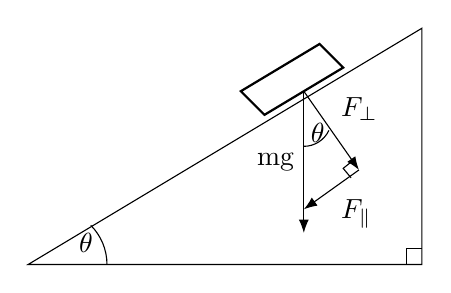
\begin{tikzpicture}
                \draw (0,0) -- (5,0) -- (5,3) -- cycle;
                \draw (1,0) arc (0:45:20pt) node[anchor=east,midway] {$\theta$};
                \draw (4.8,0) -- (4.8,0.2) -- (5,0.2);
                \draw[thick] (3,1.9) -- (4,2.5) -- (3.7,2.8) -- (2.7,2.2) -- cycle;
                \draw[-Latex] (3.5,2.2) -- (3.5,0.4) node[anchor=east,midway] {mg};
                \draw[-Latex] (3.5,2.2) -- (4.2,1.2) node[anchor=south west,midway] {$F_{\perp}$};
                \draw[-Latex] (4.2,1.2) -- (3.5,0.7) node[anchor=north west,midway] {$F_{\parallel}$};
                \draw (4.1,1.1) -- (4,1.22) -- (4.1,1.3);
                \draw (3.5,1.5) arc (270:335:10pt) node[anchor=south east,yshift=-8pt,xshift=2pt] {$\theta$};
            \end{tikzpicture}
        \end{center}
        \textit{*defining the positive direction as down the slope} \\
        Time to stop:
        \begin{align*}
            t &= \frac{2s}{u+v} = \frac{2\times1}{100+0} = 0.02\,s.
        \end{align*}
        \part Find the angle of incline of the slope.\quad[5 marks]

        Deceleration of the train:
        \begin{align*}
            a = \frac{v-u}{t} = \frac{0-100}{0.02} &= -5\times10^3\,\text{km\,hr}^{-2},\\
            =-5\times10^3\times\frac{1000}{3600^2} &= -0.39\,\text{m}\,s^{-2}.
        \end{align*}
        Balancing the forces on the train for $\theta$:
        \begin{align*}
            F_{\parallel} - F_{br} &= mg\sin\theta - F_{br} = ma, \\
            g\sin\theta &= a + \frac{F_{br}}{m},\\
            \sin\theta &= 0.039 \implies \theta = 2.3^\circ.
        \end{align*}
    \end{parts}

    \newpage
\begin{center}
\fbox{\parbox{5.5in}{\centering
\textbf{Section B: Rainbows}}}
\end{center}

\question What is your favourite colour of the rainbow and why? Write about three sentences.

Purple is definitively the best colour of the rainbow, and I will now outline with scientific evidence why this is so. 
Welcome to my TED talk. 

For centuries, the bourgeoisie across the world have chosen to dye their fancy clothing (bought no doubt at the expense of the working classes of their societies) with colours such as purple. 
Despite what we may think of the bourgeoisie, their choice in colour was still a clever one. 
What other colour invokes such a sense of beauty and nobility as that of purple?
The difficulty in procuring such a dye only made it even more precious, and yet, despite the difficulty, the ruling classes were determined that this was one of the colours that they must wear to symbolise their `upper station'.
No other colour throughout history has been as sought after or as coveted as purple. 
Surely centuries of human culture and development cannot be wrong in lusting after such a colour?
We must now rejoice, however, that this colour is no longer limited to the bourgeoisie and we can all wear its glorious hues (though this may cause difficulties in distinguishing the rich when the Revolution comes).

What is a more beloved time of day than the twilight? (There was even a whole book series about it!)
Can you guess why the twilight sky is so adored?
Correct. 
The purple tones of the sky give off such beauty and tranquility that we cannot help but stare and allow our souls to be soothed. 
You may challenge this point of view with another colour of sky, but you will not last long. 
A red sky? Death. A blue sky? You've probably got sunburn. A yellow sky? That's just the sun, look further around. A green sky? You've either been watching Pirates of the Caribbean or there is an incoming Death Star strike; you choose which is worse. 
The purple hues of a twilight sky can only give you happy thoughts and positive connotations, whereas any other colour will clearly bring about your doom. 

What colour has a movie made about it? The Colour Purple. 
That one was obvious. 
What is the colour of Scotland's national flower? (Thistle be an easy one) Purple! 

Here, I have presented definitive proof of the greatness of purple by drawing a mind-map of all the wonderful connotations we all have for this beautiful colour. 
It is impossible to dispute my findings here, so don't try it. I have the high ground. 

\end{questions}

\end{document}


